%% =============================
%%      IMPORTANTE
%% ESTE ARQUIVO DEVE ESTAR SALVO COMO
%%      UTF - 8
%% =============================

% ----------------------------------------------------------
% Este capítulo é parte integrante do arquivo mestre
% Relatorio_TCC_Mestrado_Base_VERSÃO_SUBVERSÃO_FHZ
% ----------------------------------------------------------
\definecolor{pastelgray}{rgb}{0.81, 0.81, 0.77}

% ----------------------------------------------------------
\chapter{Introduction}
\label{chap:introduction}
% ----------------------------------------------------------

In recent years, there has been a significant rise in the interest of using Artificial Intelligence (AI), particularly Machine Learning (ML) and Deep Learning (DL), in diverse fields such as fluid dynamics and turbulence modeling. The integration of data-driven approaches with computational fluid dynamics (CFD) are promising for achieving faster predictions and optimizations previously unnimaginable. The transformation of fluid dynamics through ML and data-driven methods yields valuable new insights into complex flow phenomena and facilitates the development of efficient frameworks for characterization, prediction, and control, as exemplified by key contributions discussed in this review.

\section{Bibliography Review}

A bibliometric review was conducted in Scopus and Web of Science databases. The goal was to identify the most relevant works within the scope of our current research themes while ensuring a broad search. To accomplish this, a series of boolean operations were used, resulting in the following search query:

\begin{lstlisting}[
    breaklines, 
    label={lst:query},
    basicstyle=\ttfamily, 
    columns=fullflexible, 
    keepspaces=true,
    backgroundcolor=\color{pastelgray}, 
    breakatwhitespace=true, 
    numbers=none,
    caption={Search query used to filter relevant works in the in \textit{Scopus} and \textit{Web of Science} databases.},
    captionpos=b
    ]
    ("flow reconstruction" OR "field reconstruction" OR "reconstruction" OR "flow field" OR "flow fields") AND ("surrogate" OR "metamodel" OR "meta model" OR "order reduction" OR "reduced order" OR "PCA" OR "POD" OR "SVD" OR "principal component analysis" OR "singular value decomposition" OR "proper orthogonal decomposition" OR "machine learning" OR "neural network" OR "neural networks" OR "gaussian process" OR "kriging" ) AND ("compressible" OR "viscous" OR "turbulent" OR "RANS" OR "Navier-Stokes" OR "inviscid" OR "Euler" OR "fluid dynamic" OR "fluid dynamics") AND ("data-driven" OR "data driven")    
\end{lstlisting} 

This resultant query assures the exploration of the area, covering main topics related to flow reconstruction, dimensionality reduction, surrogate modeling, and fluid dynamics methods. A schematic  representation of search strategy is provided to illustrate the logical structure of the query, highlighting the interaction of various concepts and methodologies involved.

\begin{figure}
\begin{circuitikz}\draw
    (-5,2.9) node (flow_reconsctruction) {flow reconsctruction}
    (-5,2.5) node (field_reconsctruction) {field reconsctruction}
    (-5,2.1) node (reconsctruction) {reconsctruction}
    (-5,1.7) node (flow field) {flow field}
    (-5,1.3) node (flow fields) {flow fields}
    (1,2.1) node[or port, yscale=1.75, xscale=1.75, number inputs=5] (myor1) {\fontsize{10}{10}\selectfont OR}
    (flow_reconsctruction) -- (myor1.in 1)
    (field_reconsctruction) -- (myor1.in 2)
    (reconsctruction) -- (myor1.in 3)
    (flow field) -- (myor1.in 4)
    (flow fields) -- (myor1.in 5)

    (-5,0.5)  node (surrogate) {surrogate}
    (-5,0.1) node (metamodel) {metamodel}
    (-5,-0.3) node (meta_model) {meta model}
    (-5,-0.7) node (order_reduction) {order reduction}
    (-5,-1.1) node (PCA) {PCA}
    (-5,-1.5)  node (POD) {POD}
    (-5,-1.9) node (SVD) {SVD}
    (-5,-2.3) node (principal_component_analysis) {principal component analysis}
    (-5,-2.7) node (proper_orthogonal_decomposition) {proper orthogonal decomposition}
    (-5,-3.1) node (machine_learning) {machine learning}
    (-5,-3.5) node (neural_network) {neural network}
    (-5,-3.9) node (neural_networks) {neural networks}
    (-5,-4.3) node (gaussian_process) {gaussian process}
    (-5,-4.7) node (kriging) {kriging}
    (2.5,-2.1) node[or port, yscale=5.0, xscale=3.0, number inputs=14] (myor2) {\fontsize{3.5}{0.5}\selectfont OR}
    (surrogate) -- (myor2.in 1)
    (metamodel) -- (myor2.in 2)
    (meta_model) -- (myor2.in 3)
    (order_reduction) -- (myor2.in 4)
    (PCA) -- (myor2.in 5)
    (POD) -- (myor2.in 6)
    (SVD) -- (myor2.in 7)
    (principal_component_analysis) -- (myor2.in 8)
    (proper_orthogonal_decomposition) -- (myor2.in 9)
    (machine_learning) -- (myor2.in 10)
    (neural_network) -- (myor2.in 11)
    (neural_networks) -- (myor2.in 12)
    (gaussian_process) -- (myor2.in 13)
    (kriging) -- (myor2.in 14)

    (-5,-5.5) node (compressible) {compressible}
    (-5,-5.9) node (viscous) {viscous}
    (-5,-6.3) node (turbulent) {turbulent}
    (-5,-6.7) node (RANS) {RANS}
    (-5,-7.1) node (Navier_Stokes) {Navier-Stokes}
    (-5,-7.5) node (inviscid) {inviscid}
    (-5,-7.9) node (Euler) {Euler}
    (-5,-8.4) node (fluid_dynamic) {fluid dynamic}
    (-5,-8.9) node (fluid_dynamics) {fluid dynamics}
    (1.5,-7.15) node[or port, yscale=3.35, xscale=3.0, number inputs=9] (myor3) {\fontsize{4.375}{4.375}\selectfont OR}
    (compressible) -- (myor3.in 1)
    (viscous) -- (myor3.in 2)
    (turbulent) -- (myor3.in 3)
    (RANS) -- (myor3.in 4)
    (Navier_Stokes) -- (myor3.in 5)
    (inviscid) -- (myor3.in 6)
    (Euler) -- (myor3.in 7)
    (fluid_dynamic) -- (myor3.in 8)
    (fluid_dynamics) -- (myor3.in 9)
    
    (4.5,-2.1) node[and port, number inputs=3] (myand1) {AND}
    (myor1.out) -- (myand1.in 1)
    (myor2.out) -- (myand1.in 2)
    (myor3.out) -- (myand1.in 3)

    (6.0,-2.1) node (final_query) {final query}
    (myand1.out) -- (final_query);
\end{circuitikz}
\caption{Boolean circuit representation of the search query of Listing \ref{lst:query}.}
\label{fig:query}
\end{figure}
Following the bibliometric analysis, we examined the retrieved literature to consolidate key findings and insights relevant to our study. Subsequently, we provide a summary of the substantial discussion and literature review, focusing on various machine learning applications in fluid dynamics, the effectiveness of dimensionality reduction techniques and the future potential of such technologies in real-world applications. We present a the selection of contributions identified during the review process.

\begin{figure}[h]
    \centering
    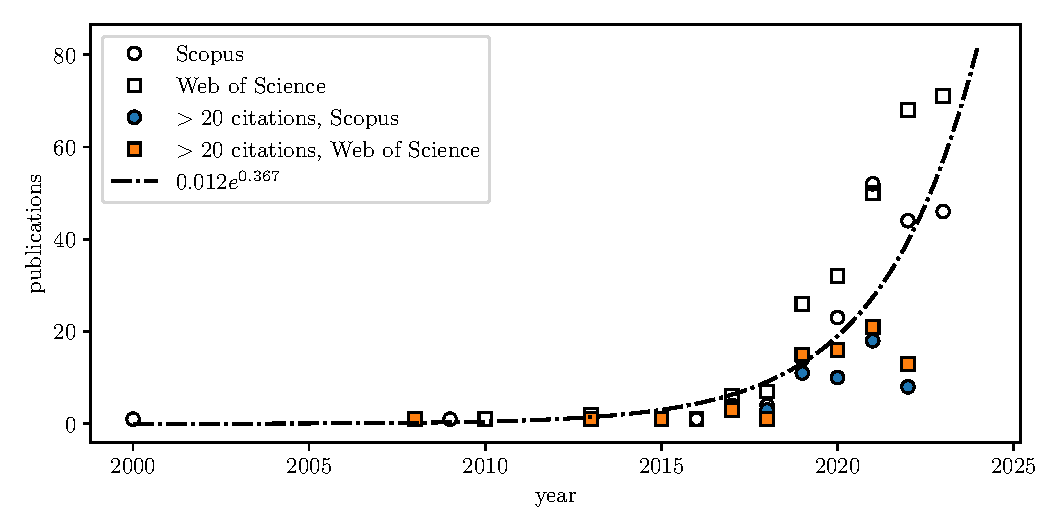
\includegraphics[width=\textwidth]{Figuras/bibliometric_review.pdf}
    \caption{Results of using the search query of Listing \ref{lst:query} in \textit{Scopus} and \textit{Web of Science}. This figure displays how new this field of study is, and it also reveals an exponential rise in publications each year, both in terms of raw data and also when considering the more notable publications (those with more than 20 citations).}
    \label{fig:bibliometric_review}
\end{figure}

\citet{Bright2013} introduced a compressive sensing machine learning strategy for fluid dynamics, demonstrating efficient characterization of flow around a cylinder using sparse pressure measurements. This work paved the way for data-driven strategies in fluid mechanics, highlighting the potential of combining dimensionality reduction and convex optimization for flow field reconstructions. 

\citet{Zhang2015} advanced the field by examining machine learning models for data-driven turbulence modeling, focusing on reconstructing functions from high-fidelity simulation data. Their work addresses the importance of selecting appropriate learning algorithms and identified factors influencing model output, suggesting the strong potential of ML in augmenting traditional turbulence modeling approaches.

\cite{Wan2017a} introduced a reduced-space Gaussian Process Regression (GPR) for data-driven probabilistic forecasts of chaotic dynamical systems. By incorporating local interpolation error and phase space truncation uncertainties, they offered a novel perspective on forecasting complex systems, showing of the broader applicability of machine learning in uncertainty quantification and prediction within fluid dynamics.

In another work, \citet{Wang2017a} utilized detached eddy simulation (DES) and proper orthogonal decomposition (POD) to investigate unsteady flow behavior in steam turbine control valves. Their approach effectively demonstrated the synergy between simulation techniques and data-driven methods in understanding complex flow behaviors and their impact on valve performance.

The progression toward using evolutionary algorithms for the development of algebraic stress models, as explored by \citet{Weatheritt2017c}, further illustrates how machine learning methods can optimize fluid dynamics modeling beyond conventional approaches. This method offers a framework for creating tangible mathematical expressions of fluid dynamics phenomena, enhancing both accuracy and interpretability of turbulence models.

\citet{Bolton2019b} explored the use of convolutional neural networks for ocean data inference and subgrid parameterization. Their work demonstrated the capacity of deep learning models to replicate and predict subgrid-scale dynamics in oceanographic studies, marking a significant step forward in the use of ML for environmental fluid mechanics.

\citet{Demo2019c} combined POD with the active subspace property to enhance reduced order models (ROMs) for fluid dynamics. This innovative approach not only improved the accuracy of ROMs but also significantly reduced the computational cost of simulations .

Looking into fire safety, \cite{Hodges2019c} applied transpose convolutional neural networks for predicting compartment fire behaviors, showcasing how deep learning can offer rapid and robust predictions essential for safety assessments.

\cite{Jayaraman2019a, Zhu2019} delved into sparse reconstruction of fluid flows, demonstrating how learning from high-dimensional data can address challenges in aerodynamics and turbulence modeling. These contributions highlight the evolving landscape of fluid dynamics research, where data-driven methods are increasingly critical for advancing our understanding and capabilities in analyzing, predicting, and controlling fluid flows.

Complementing this, \citet{Geneva2020c} introduced a multi-fidelity deep learning model for surrogate modeling of turbulent flows. Their model, employing conditional invertible neural networks, marked a significant advance in capturing the complex dynamics of high Reynolds number flows, including turbulent wake behind bluff bodies. Such multi-fidelity approaches exhibit immense potential in providing accurate, yet computationally efficient, predictions of turbulent fluid flows.

On the search for efficient methodologies in data-driven predictions,\citet{Erichson2020b} presented a novel approach utilizing shallow neural networks for the reconstruction of fluid flow fields with limited sensors. Their methodology surpassed traditional modal approximation techniques in fluid mechanics, illustrating the effectiveness of neural networks in achieving high-quality flow field estimations from sparse datasets.

Another interesting application of ML is the reconstruction of velocity fields from experimental images, \cite{Barwey2022c}. They utilized CNNs to morph time-resolved experimental OH-PLIF images into corresponding three-component planar PIV fields, highlighting the powerful capability of CNNs in decoding complex fluid dynamics from experimental data, and to fill the gap between different types of experimental data, enhancing interpretability and utility.

The fast prediction of flow fields around airfoils using DL was tackled by \citet{Sekar2019}. By combining CNN and Multilayer Perceptron networks, they have demonstrated deep learning could offer fast and accurate flow field predictions, cutting down the time needed by traditional Navier-Stokes numerical solvers. This study highlighted the scalability and efficiency of using deep learning for aerodynamics research.

In a review that follows the above developments, \citet{Zhu2022a} provided an analysis of ML applications in multiphase flows and reactors. They enphasized the potential of ML in developing closure models, optimizing reaction conditions, and enhancing our understanding of complex flow and reaction mechanisms.

Further, the integration of Generative Adversarial Networks (GANs) in flow field prediction has received considerable attention. For instance, \citet{WU2022a} presented a data augmented GAN (daGAN) for efficient and accurate prediction of flow fields around airfoils, even with sparse training data. This work emphasizes the potential of GANs in augmenting existing datasets and enhancing the accuracy of prediction models, fostering advancements in aerodynamics and related fields.

\citet{Peters2023} presented an initial investigation into the application of a data-driven surrogate modeling technique, emphasizing rotor design applications. Their work demonstrated the capability of a proper orthogonal decomposition (POD)-based reduced-order model (ROM) derived from computational fluid dynamics (CFD) data for predicting rotor distributed loads across varying conditions with significantly reduced computational costs. On a related work, \citet{Lee2024} introduces an improved parametric model order reduction approach, particularly tailored for fluid-structure interaction analysis. Their methodology, a nonintrusive parametric model order reduction approach which combines POD with machine learning, demonstrated good performance on benchmark problems like the two-dimensional airfoil, showing of the potential in integrating machine learning with traditional model reduction techniques for fluid-structure interaction analysis.

In the realm of turbulence modeling, \citet{Li2024} illustrates the effectiveness of diffusion models (DMs) in reconstructing turbulent flow dynamics, showing superiority over classical generative adversarial networks (GANs) in both point-wise reconstruction and the statistical properties of inferred fields. \citet{Fujio2023} further explores Gaussian process latent variable modeling in conjunction with deep learning for robust predictions of scramjet flowfields, their ROM-based predictions showed the potential of the use of data-driven techniques for fast and accurate aerospace simulations.

In a similar way, \citet{Li2023a} developed a machine learning framework for modeling turbulent mixing flows within mechanically agitated vessels. Their approach, made use of supervised learning algorithms, show the potential of minimal data requirements to predict complex flow dynamics accurately, this could inspire further exploration into data-driven frameworks for multiphase flow systems. Additionally, \cite{Jin2024} introduced an extended dynamic mode decomposition framework integrated with an invertible dictionary learning, the method achieved enhanced performance in capturing the essential dynamics of data-driven systems. This work exemplifies the progress being made towards refining data-driven methodologies for better capturing physical systems' dynamics.

The exploration of indoor airflow fields through operator neural networks \cite{Gao2024}, represents a significant advance toward the fast prediction and efficient environmental control within building environments. Innovative computational strategies is further exemplified in \citet{Min2024}, where data-driven surrogate models where used in predicting the pressure fields around parallel twin cylinders, paving the way for computational savings in fluid dynamics (CFD) simulations.

Furthermore, the correction of coarse grid CFD simulations using machine learning post-processing tools as detailed by \citet{Kiener2023} lead to promising in blending data-driven methodologies with traditional simulation techniques to achieve greater accuracy in aerodynamic analysis. The time-variant prediction of flow over an airfoil using deep neural network models, as proposed by \cite{Peng2020b}, alongside the research by \citet{Reinbold2021d} on learning models from noisy and incomplete experimental data, show the transformative impact of machine learning in modeling complex physical phenomena from experimental observations.

Similarly, the employment of supervised learning for physical field reconstruction \cite{Liu2021c}, and the novel method of analyzing unsteady flow fields using deep autoencoders in \cite{Omata2019c}, illustrate the expanding frontiers of data-driven methods in capturing the intricacies of fluid dynamics. \citet{Liu2021c} introduced a method using deep convolutional neural networks (CNNs) to predict physical fields in a heat transfer problem, showcasing the effectiveness of data-driven approaches in capturing complex flow behaviors. Similarly, \citet{Riel2021c} developed a PINN framework to infer variations in drag across glacier beds, demonstrating the versatility of PINNs in geophysical flow applications. These studies underscore the adaptability of PINNs in accurately modeling fluid dynamics across diverse domains.

The work on neural network-based eddy-viscosity correction for RANS simulations by \cite{Volpiani2022}, and the challenges in fast flow field prediction of hydrofoils tackled through deep learning by \cite{Li2023}, offer valuable insights into the integration of computational techniques with machine learning for enhanced fluid dynamics modeling.

The afforementioned recent studies represent only a fraction of ongoing efforts to merge data-driven methodologies with fluid dynamics, promising to revolutionize predictions and control in fields like aerospace and environmental sciences. The literature review highlights a dynamic new era where machine learning (ML) and deep learning (DL) are increasingly applied, offering fresh insights, faster simulations, and enhanced predictive capabilities for complex flow phenomena. This integration of data-driven approaches with traditional fluid dynamics marks a revoltion, driving advancements in simulation efficiency. This body of work illuminates current trends and methodologies and also sets the stage for further exploration and discourse in the field.